\documentclass[12pt,a4paper]{article}
\usepackage[margin=1in]{geometry}
\usepackage{amsmath,amssymb}
\usepackage{booktabs}
\usepackage{graphicx}
\usepackage{hyperref}
\usepackage{enumitem}
\usepackage{float}

\title{Implementation of Pose Estimation on SO(3) using the Passive Mahony Filter}
\author{Armaan Raisinghani and Shikhraj Singh}
\date{\today}

\begin{document}
\maketitle

\section*{Submission Links}
\begin{itemize}[leftmargin=1.5em]
    \item GitHub repository: \url{<PASTE_GITHUB_LINK_HERE>}
    \item YouTube demonstration video: \url{<PASTE_YOUTUBE_LINK_HERE>}
\end{itemize}

\section{Assignment Scope}
This submission focuses on implementing the passive Mahony nonlinear complementary filter on $SO(3)$ using IMU and magnetometer data. The required supporting steps are:
\begin{enumerate}[leftmargin=1.5em]
    \item Sensor interfacing (gyroscope, accelerometer, magnetometer), frame remapping to a common inertial convention (ENU), and calibration.
    \item Gyro integration on $SO(3)$ using the exponential map / Rodrigues formula.
    \item TRIAD implementation using accelerometer and magnetometer as a rotation measurement input.
    \item Passive Mahony filter on $SO(3)$ with gyro-bias estimation.
    \item Quaternion output and live 3D visualization for passive-filter validation.
\end{enumerate}

\section{Contribution Clarification}
The Python visualization code and a major portion of the filter framework were provided as part of the course resources. This submission focuses on adaptation and validation work, specifically:
\begin{itemize}[leftmargin=1.5em]
    \item ENU frame remapping and consistent axis/sign alignment,
    \item sensor calibration and calibration-constant integration,
    \item passive-filter parameter tuning and runtime checks,
    \item end-to-end testing, visualization setup, and analysis of behavior.
\end{itemize}

\section{Implementation Summary}
\subsection{Sensor Interfacing and ENU Alignment}
All sensor readings were remapped into a consistent ENU-compatible body convention before fusion. In particular:
\begin{itemize}[leftmargin=1.5em]
    \item Gyroscope channels were remapped to match the chosen body-axis definition used in the visualization.
    \item Accelerometer and magnetometer channels were remapped with sign and axis corrections so all modules used the same frame convention.
    \item Initial calibration was performed with the IMU body frame aligned with the chosen inertial reference.
\end{itemize}

\subsection{Calibration}
\begin{itemize}[leftmargin=1.5em]
    \item Gyroscope: static bias estimated from averaged stationary samples.
    \item Accelerometer: static offset check under known gravity direction.
    \item Magnetometer: hard-iron and soft-iron compensation using calibration matrix and bias vector. This matrix was provided to us.
\end{itemize}

\subsection{Gyro Integration on $SO(3)$}
The attitude kinematics were integrated using
\[
R_{k+1} = R_k\exp(\Omega_k^{\times}\Delta t),
\]
with Rodrigues approximation for matrix exponential:
\[
\exp(\theta K) = I + \sin(\theta)K + (1-\cos\theta)K^2,
\]
where $\theta = \|\Omega\|\Delta t$ and $K$ is the unit-axis skew matrix.
The practical procedure used in each loop was:
\begin{enumerate}[leftmargin=1.5em]
    \item Read raw gyroscope channels and convert from deg/s to rad/s.
    \item Apply ENU remapping and subtract the estimated static bias vector.
    \item Build $\Omega^{\times}$ through the skew-symmetric operator.
    \item Update $R$ with the exponential-map step at fixed sample time $\Delta t$.
    \item Reuse this rotation both for visualization and as the propagation model inside the passive filter pipeline.
\end{enumerate}

\subsection{TRIAD Measurement Block}
TRIAD (provided baseline structure) was configured with accelerometer as the first vector and magnetometer as the second vector. This generated the rotation measurement used by the passive Mahony correction step.
Given normalized body-frame vectors $a_b$ and $m_b$, and normalized reference vectors $a_r$ and $m_r$, TRIAD was computed using orthonormal bases:
\[
q_b = a_b,\quad r_b = \frac{q_b \times m_b}{\|q_b \times m_b\|},\quad s_b = q_b \times r_b,
\]
\[
q_r = a_r,\quad r_r = \frac{q_r \times m_r}{\|q_r \times m_r\|},\quad s_r = q_r \times r_r.
\]
Then
\[
R_{\text{triad}} = [q_r\ r_r\ s_r][q_b\ r_b\ s_b]^\top.
\]
The practical procedure was:
\begin{enumerate}[leftmargin=1.5em]
    \item Apply accelerometer and magnetometer remapping to the common ENU-compatible convention.
    \item Normalize both vectors to use directional information only.
    \item Compute body/reference triads and construct $R_{\text{triad}}$.
    \item Use $R_{\text{triad}}$ as the instantaneous measurement matrix for passive-filter correction.
\end{enumerate}
This block is sensitive to magnetic disturbance and linear acceleration, so it was treated as a correction/reference signal rather than the final estimate.

\subsection{Passive Mahony Filter}
The passive nonlinear complementary filter on $SO(3)$ code path (from provided base code) was configured and tuned with
\begin{itemize}[leftmargin=1.5em]
    \item attitude correction from rotation error projection,
    \item integral gyro-bias estimation,
    \item proportional correction in the angular-rate update.
\end{itemize}
Quaternion streams were published for visualization in this order: \textbf{Gyro}, \textbf{TRIAD}, \textbf{Passive Mahony}. Gyro and TRIAD are included as intermediate/supporting references for debugging and validation.
Using propagated estimate $R_{\text{est}}$ and TRIAD measurement $R_{\text{triad}}$, the rotation error was formed as
\[
R_E = R_{\text{est}}^\top R_{\text{triad}}, \quad
\mathcal{P}_{\text{anti}} = \frac{1}{2}(R_E - R_E^\top),
\]
and mapped to vector form
\[
w = [\mathcal{P}_{\text{anti}}(3,2),\ \mathcal{P}_{\text{anti}}(1,3),\ \mathcal{P}_{\text{anti}}(2,1)]^\top.
\]
Bias and corrected angular-rate updates were applied as:
\[
\hat b_{k+1} = \hat b_k - k_i\,\Delta t\,w,
\]
\[
\Omega_{\text{corr}} = \Omega - \hat b + k_p\,w,
\]
followed by $R_{\text{est},k+1} = R_{\text{est},k}\exp(\Omega_{\text{corr}}^{\times}\Delta t)$.
The tuning workflow was: start with small $k_i$ to avoid slow oscillatory bias drift, increase $k_p$ until correction was responsive but not noisy, then iterate while checking heading stability and transient response in the live visualization.

\section{Visualization Setup}
The provided Python monitor (pygame), with label and stream mapping edits, displays three active cubes corresponding to:
\begin{enumerate}[leftmargin=1.5em]
    \item Gyro integration output,
    \item TRIAD output,
    \item Passive Mahony output.
\end{enumerate}
This supports side-by-side validation of the passive estimator against its input/reference blocks under identical motion.

\section{Analysis and Observations}
\subsection{Gyro-only integration}
\begin{itemize}[leftmargin=1.5em]
    \item Without bias-correction, the gyro-only estimate starts drifting within seconds, due to the nature of the IMU bias and the integration process.
    \item Short-term motion is smooth and responsive, but long-term stability is poor.
    \item With bias correction, the reading is reliable only for up to 60 seconds, after which, even when left stable, there is anoticable drift of $\textgreater 30$\textdegree s.
    \item Passive Mahony output is used as the reference estimate for comparison in the analysis.
\end{itemize}

\begin{figure}[H]
    \centering
    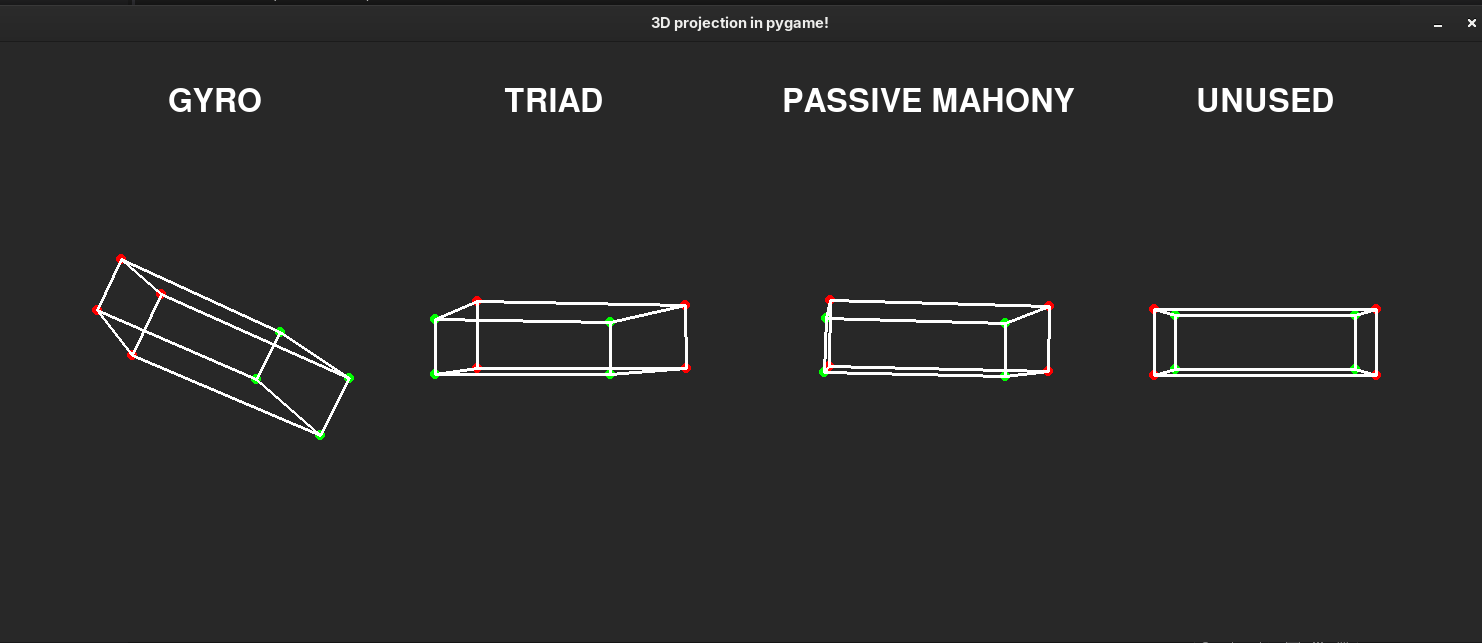
\includegraphics[width=0.85\linewidth]{images/gyro.png}
    \caption{Gyro-only response, compared against Passive Mahony reference behavior.}
    \label{fig:gyro_analysis}
\end{figure}

\subsection{TRIAD}
The following behaviors were used to interpret passive-filter performance:
\begin{itemize}[leftmargin=1.5em]
    \item TRIAD is always aligned with the true gravity and north vector, so it provides a true reference.
    \item However, it is noisy and can be unstable even at rest due to the noisiness of the accelerometer and magnetometer sensor readings.
\end{itemize}

\begin{figure}[H]
    \centering
    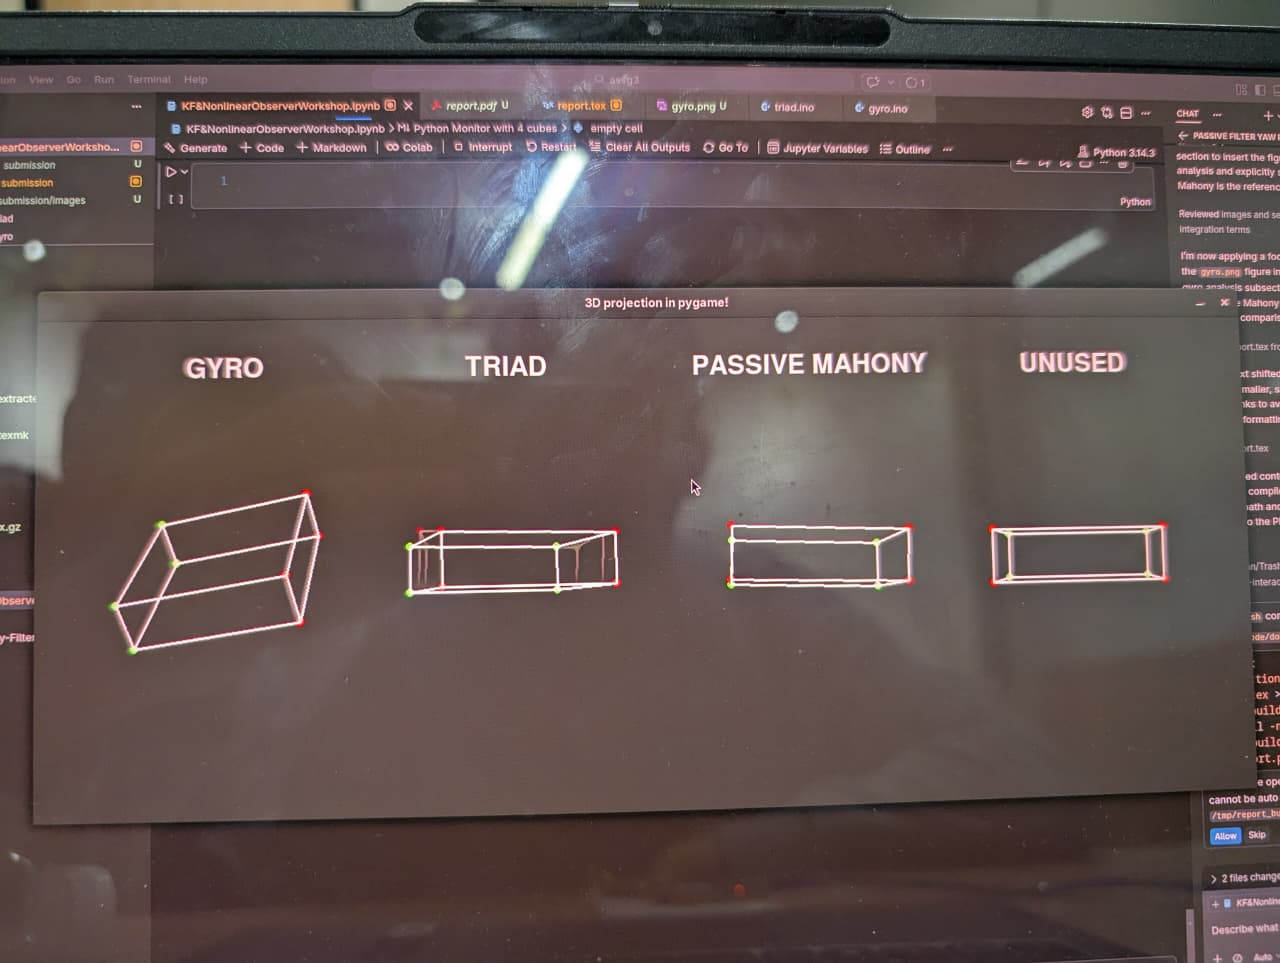
\includegraphics[width=0.85\linewidth]{images/triad.png}
    \caption{TRIAD output shown as a long-exposure shot taken from a camera, highlighting how shaky the estimate was.}
    \label{fig:triad_analysis}
\end{figure}

\subsection{Passive Mahony Filter}
The following behaviors were used to interpret passive-filter performance:
\begin{itemize}[leftmargin=1.5em]
    \item Passive mahony was by far the most accurate and stable estimate, with good transient response and heading stability.
    \item The passive filter was able to reject gyro drift and maintain a stable heading reference, even under moderate motion.
    \item However, it was not completely perfect. After strong shaking and some time at rest, it would still show some slow drift of $\approx 5$\textdegree/s yaw, which is likely due to the limitations of the sensor calibration and the correction gains.

\end{itemize}

\begin{figure}[H]
    \centering
    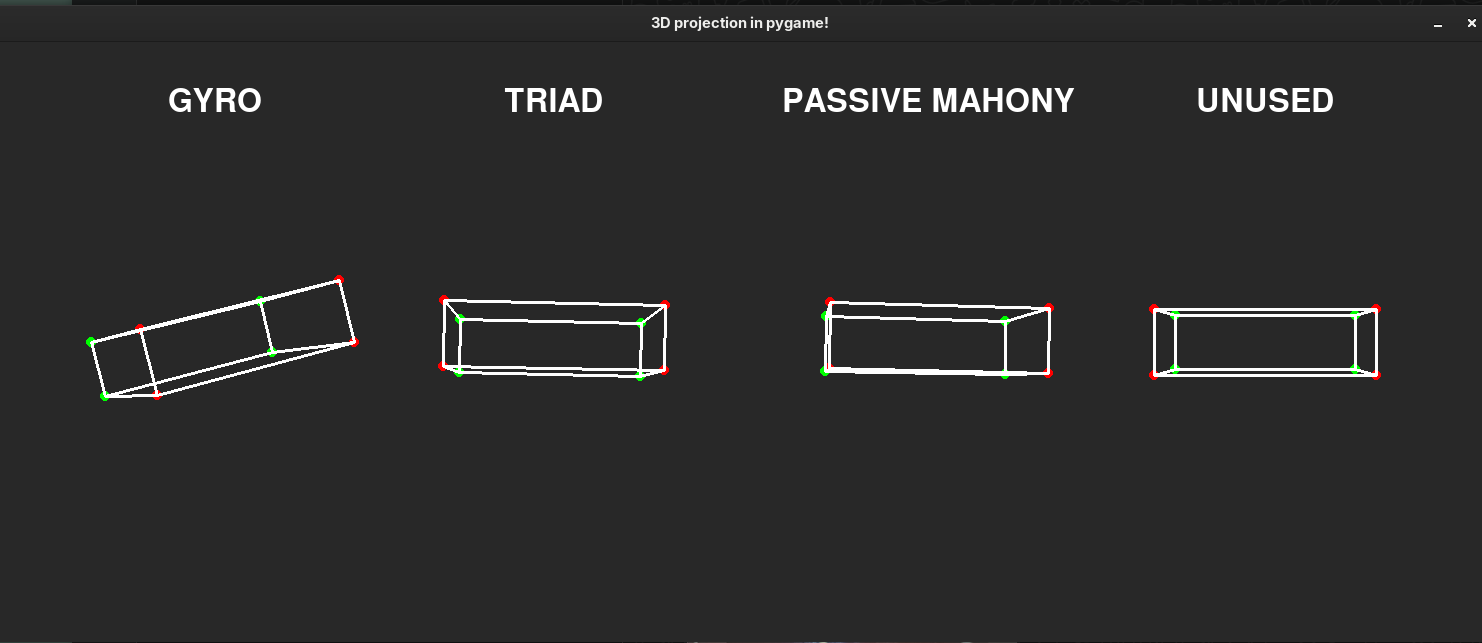
\includegraphics[width=0.85\linewidth]{images/mahony.png}
    \caption{Passive Mahony filter output under the same motion sequence.}
    \label{fig:mahony_analysis}
\end{figure}


\subsection{Final Conclusion}
The passive Mahony filter was successfully implemented and it provided a significant improvement in attitude estimation stability and accuracy compared to gyro-only integration, while effectively using the TRIAD measurement as a correction reference. The live visualization was instrumental in tuning the filter parameters and understanding the behavior of each component under different motion conditions.


\section*{Appendix: Files Submitted}
\begin{itemize}[leftmargin=1.5em]
    \item Adapted Arduino sketches for gyro integration, TRIAD block, and passive Mahony pipeline.
    \item Provided Python visualization notebook with assignment-specific label/stream mapping updates.
    \item This report (PDF generated from \texttt{report.tex}).
\end{itemize}

\end{document}
